\chapter{Road Mapping}
\section{Overview}
\subsection{Context}
Objective of year 4 is to bring together all your knowledge from your undergraduate courses and see how it can be applied to real practical problems. Graduate level courses put the emphasis on the student to find and read around the material.
\begin{itemize}
    \item First, we will explore what we mean by the words ``extreme pressure'', ``extreme chemistry'' and ``extreme temperature''
          \begin{itemize}
              \item \dots by looking at a number of examples
          \end{itemize}
    \item Structure of the courses - the role of the professor and your role
    \item Formalisation of these definitions and classifications
    \item How does industry deal with these problems
\end{itemize}
\subsection{Course assessment}
\textbf{Assessments}
\begin{enumerate}
    \item Coursework (30\%) - January
    \item Group Project (40\%) - end of March
    \item Laboratory class (30\%) - February
\end{enumerate}
1, 2, 3 will cover the three themes of pressure, temperature and chemistry.
\begin{table}[htbp]
    \centering
    \begin{tabular}{@{}llll@{}}
        \toprule
                      & \textbf{2018-2019}    & \textbf{2019-2020}            & \textbf{2020-2021}            \\
        \midrule
        Exam          & Extreme Pressure      & Extreme Temperature           & CW Extreme Temperature        \\
        Group Project & Extreme Temperature   & Extreme Pressure              & Extreme Pressure              \\
        Laboratory    & Corrosion (chemistry) & Extreme chemistry (corrosion) & Extreme chemistry (corrosion) \\
        \bottomrule
    \end{tabular}
    \caption{Table to show themes of assessments in previous years.}
\end{table}
\subsection{Group project - extreme pressure 2019 / 2020}
You must choose which problem you are interested in and we will organise you into groups. We will have a fortnightly session to discuss through the term and give you help. We will be running training sessions so that everyone has a chance to learn a bit about CFD. Need to raise the game from last year - tended to have a late start.
\subsection{Course structure}
4 teaching blocks:
\subsubsection{Block 1}
Lectures 1-4:
\begin{itemize}
    \item Setting the scene, framework and terminology
    \item Investigative tools used to solve hard problems
    \item Key concepts for molecular scales (chemistry and materials)
    \item Key concepts for continuum scales (fluid mechanics, solid mechanics and structures)
\end{itemize}
\subsubsection{Block 2}
Lectures 5-8: Extreme Pressure.
\begin{itemize}
    \item Static cases
          \begin{enumerate}
              \item High pressure: bottom of the ocean, pressure vessels
              \item Low pressure: space, cavitation
          \end{enumerate}
    \item Unsteady cases
          \begin{enumerate}
              \item High pressure: gas flows, AIV, explosions (nuclear), liquid flows, VIV, TIV
              \item Low pressure: cavitation
          \end{enumerate}
\end{itemize}
\subsubsection{Block 3}
Lecture 9-12: Extreme Chemistry.
\begin{itemize}
    \item Slow chemistry
          \begin{enumerate}
              \item Corrosion
          \end{enumerate}
    \item Fast chemistry
          \begin{enumerate}
              \item Fuel cells
              \item Combustion
          \end{enumerate}
    \item Application section: manufacturing, design and testing
\end{itemize}
\subsubsection{Block 4}
Lecture 13-16: Extreme Temperature.
\begin{itemize}
    \item Static cases
          \begin{enumerate}
              \item High temperature: fire, manufacturing, coatings
              \item Low temperature: arctic, LNG transport
          \end{enumerate}
    \item Unsteady cases
          \begin{enumerate}
              \item Thermal shocks
          \end{enumerate}
\end{itemize}
\section{Engineering in extreme environments}
What do we mean by these words?
\begin{quoting}
    The phrase "engineering in extreme environments" relates to the study, design, and implementation of engineering solutions that can withstand and function optimally under extremely harsh or atypical conditions. These conditions are characterized by extreme pressure, extreme temperature, and extreme chemical environments, all of which present unique challenges that can significantly affect the performance and durability of materials and systems.

    Specifically:

    Extreme Pressure: Engineering in high-pressure environments often involves deep-sea, subterranean or aerospace applications, where the equipment is subjected to extraordinary pressures. This requires an in-depth understanding of material properties and structural integrity under such conditions, including factors like compression, shear stress, and deformation.

    Extreme Temperature: This refers to the ability to design and implement engineering solutions in environments with very high or very low temperatures. This might include deep-sea vents, cryogenic systems, combustion engines, or spacecraft re-entry systems. The challenges here primarily relate to thermal stress, material expansion/contraction, and maintaining operational efficiency under these temperature ranges.

    Extreme Chemistry: Engineering in extreme chemical environments requires developing materials and systems that can resist highly corrosive or reactive environments, which can include certain industrial processes, chemical plants, or hostile extraterrestrial environments. An understanding of material science, including the resistance of different materials to corrosion, oxidation, and other chemical reactions, is crucial.

    This aspect of mechanical engineering seeks to unite the foundational knowledge of mechanical engineering — such as fluid mechanics, thermodynamics, materials science, and structural analysis — with a deeper understanding of how these principles apply under extreme conditions. It typically involves rigorous testing and modelling, the use of advanced materials and coatings, and innovative design principles to ensure safety, efficiency, and longevity of engineering systems under extreme environments.

    (ChatGPT-4 2023-07-03)
\end{quoting}
\subsection{Engineering}
Engineering - a branch of science and technology concerned with the design, building, and use of engines, machines, and structures.

Focussed on the discrete elements or components that sit in an environment. We will refer to a structure throughout the course, through what we really mean is anything (engine, blade, casing, tool, system, person).
\subsection{Classification of environment}
Environment - this is just the surroundings in which an objects sits or is exposed to. There are two types of environments:
\begin{enumerate}
    \item Natural
    \item Man-made
\end{enumerate}
There has to be a physical way to communicate between the environment and the engineering structure which is usually through a surface.
\subsection{Classification of interactions}
\begin{itemize}
    \item Internal or closed problems e.g. pipe flow, IC engine
    \item Open problems e.g. fire outside, atmospheric
          \begin{itemize}
              \item Open problems represent challenges in terms of boundary conditions
          \end{itemize}
\end{itemize}
\subsubsection{Types of interactions}
\begin{itemize}
    \item Interactions are with the interfaces. What processes act on an interface?
    \item Solid surface - affected by:
          \begin{itemize}
              \item normal / tangential forces / pressure / viscous forces (high / low pressure)
          \end{itemize}
    \item Thermal effects (heating / cooling)
    \item Chemical effects (burning, corrosion)
    \item Structural changes due to forces / loading
    \item Fatigue
\end{itemize}
\subsubsection{Interfacial processes}
\begin{itemize}
    \item Temperature
    \item Stresses - solid and fluid forces
    \item Chemistry
\end{itemize}
\subsection{Classification of extremes}
Extreme has quite a few interpretations. Extreme may be something that is an outlier. The definition that we will work around is based on two types:
\begin{enumerate}
    \item based on magnitude (of a scalar or vector)
    \item how it is spread and varies spatially or temporally
\end{enumerate}
We try to tackle these broad questions using regime diagrams (Figures \ref{regimeDiagram1}, \ref{regimeDiagram2}, \ref{regimeDiagram3}).
\begin{figure}[htbp]
    \centering
    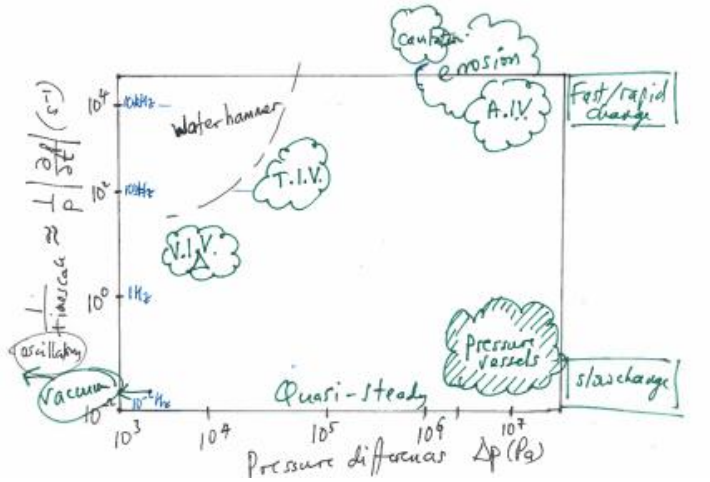
\includegraphics[width = 0.8\textwidth]{./img/figure78.png}
    \caption{Regime diagram to show different pressure environments.}
    \label{regimeDiagram1}
\end{figure}
\begin{figure}[htbp]
    \centering
    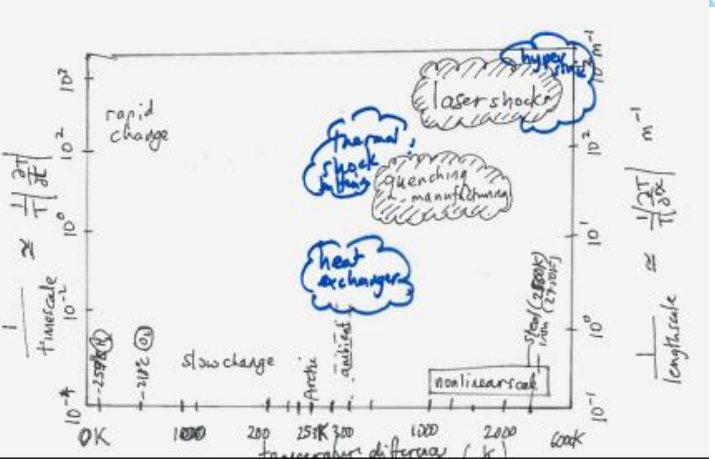
\includegraphics[width = 0.8\textwidth]{./img/figure79.png}
    \caption{Regime diagram to show different temperature environments.}
    \label{regimeDiagram2}
\end{figure}
\begin{figure}[htbp]
    \centering
    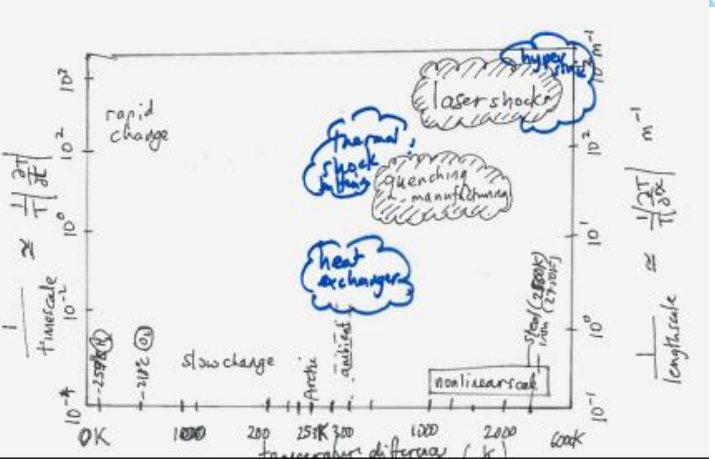
\includegraphics[width = 0.8\textwidth]{./img/figure79.png}
    \caption{Regime diagram to show different chemical environments.}
    \label{regimeDiagram3}
\end{figure}
\section{Extreme natural environments}
\begin{table}[htbp]
    \centering
    \begin{tabular}{@{}ll@{}}
        \toprule
        \textbf{Under extreme} & \textbf{Examples}            \\
        \midrule
        Pressure               & Tsunami, earthquakes, storms \\
        Temperature            & Fires, arctic                \\
        Chemistry              & Corrosion, biofouling        \\
        \bottomrule
    \end{tabular}
    \caption{Table to show example naturally extreme environments.}
\end{table}
\subsubsection{Challenges in extreme natural environments}
Main challenges are:
\begin{enumerate}
    \item Living in these external environments
    \item Working in these external environments
\end{enumerate}
\subsection{Extreme pressure}
\subsubsection{Example: deep water (high pressure)}
\begin{quoting}
    Deep underwater environments, such as those over 2000 meters below sea level, experience extreme hydrostatic pressure. This pressure can pose severe challenges to structures, equipment, and human life. For instance, habitats in deep oceans and lakes must be designed to withstand these pressures. A case in point is the Deepwater Horizon oil drilling rig, which suffered a catastrophic failure in 2010. The disaster was partly attributed to a mismanagement of high-pressure conditions approximately 1000 meters below sea level, highlighting the critical role that pressure management plays in these environments.

    (ChatGPT-4 2023-07-03)
\end{quoting}
\subsubsection{Example: hurricanes (high pressure and gustiness)}
\begin{quoting}
    Hurricanes present a convergence of extreme conditions. The high wind pressure and gustiness can lead to severe infrastructural damage. These natural disasters are formed from a convergence of tropical thunderstorms, leading to an area of low pressure with high winds blowing into the area. Over 2000 deaths have occurred due to hurricanes in the US since 2005. The combination of high pressure, high winds, and water hazards like storm surges and flooding make them a multifaceted challenge.

    (ChatGPT-4 2023-07-03)
\end{quoting}
\subsubsection{Example: earthquakes (high solid mechanical pressure)}
\begin{quoting}
    Earthquakes generate extreme solid mechanical pressures resulting from seismic activity. The vibration of the ground due to surface waves can lead to the failure and collapse of structures, making it a significant challenge for civil and structural engineers to design buildings that can withstand these forces. On average, earthquakes result in around 10,000 fatalities per year, indicating the severity of their impact and the importance of engineering designs that consider seismic activity.

    (ChatGPT-4 2023-07-03)
\end{quoting}
\subsubsection{Example: tsunami (high fluid pressure)}
\begin{quoting}
    Tsunamis represent a high-impact hazard that involves enormous fluid pressures. Generated by underwater seismic activity, landslides, or volcanic eruptions, tsunamis can travel across ocean basins and cause massive destruction when they make landfall. A devastating example of this is the 2004 Indian Ocean tsunami, which resulted in the deaths of over 230,000 people. Designing for tsunami resistance, especially in coastal areas, involves understanding and accounting for these extreme fluid pressures in order to protect structures and lives.

    (ChatGPT-4 2023-07-03)
\end{quoting}
\subsection{Extreme temperature}
\subsubsection{Example: fire on land}
\begin{quoting}
    Areas that consistently experience temperatures in excess of \SI{40}{\degree C}, often in combination with dry conditions, are prone to land fires. These high-temperature environments can cause severe challenges for both human and animal habitation, and can also lead to significant environmental damage. Land fires often result in casualties and cause extensive damage to wildlife and forests. They pose unique challenges for engineers and firefighters, who must design and implement fire prevention, containment, and extinguishing strategies. These may include fire-resistant building materials and designs, effective emergency evacuation plans, and the use of technology to predict and manage wildfires.

    (ChatGPT-4 2023-07-04)
\end{quoting}
\subsubsection{Example: arctic and antarctic}
\begin{quoting}
    These regions present extreme cold conditions that provide a unique set of challenges for both natural and human-engineered systems. Life forms such as organisms living in the ice, zooplankton and phytoplankton, fish and marine mammals, birds, land animals, and human societies have to adapt to these frigid environments. In the context of engineering, these conditions necessitate the design of structures and equipment that can withstand the low temperatures, high winds, and icy conditions prevalent in these regions. This might involve the use of special materials that retain their structural integrity at low temperatures, insulation technologies to protect against the cold, and heating systems that can operate efficiently in these conditions. Infrastructure must be designed to accommodate the challenges of ice movement and permafrost, while ensuring the safety and comfort of human inhabitants.

    (ChatGPT-4 2023-07-04)
\end{quoting}
\subsection{Extreme chemistry}
\subsubsection{Example: corrosion}
\begin{quoting}
    Corrosion is a common problem in environments where metal components are exposed to corrosive agents such as salt. Salt, particularly in the form of sea spray or road de-icing materials, can accelerate corrosion processes, leading to the deterioration and failure of metal structures and equipment. To combat this, engineers employ various protective strategies. These may include the use of special corrosion-resistant materials, protective coatings, or the application of an electro-motive force (EMF) to protect against the corrosive effects of salt.

    (ChatGPT-4 2023-07-04)
\end{quoting}
\subsubsection{Example: extreme pH (alkaline and acidic)}
\begin{quoting}
    Certain environments can present extreme pH conditions, either persistently or intermittently, that pose challenges for both natural life and engineered systems:
    \begin{itemize}
        \item Alkaline Environments: Habitats with a pH above 9, such as some soils, waters, and industrial processes, can be corrosive to certain materials and can disrupt biological processes. One interesting example is Mono Lake in California's Eastern Sierras, characterized by its highly alkaline waters. A unique feature of this environment is a soft, gelatinous microbial mat that forms on the lake's surface, demonstrating the ability of life to adapt to even these extreme conditions. For engineers, dealing with such environments might involve the use of materials that resist alkaline corrosion, or the design of systems that neutralize or manage the alkaline conditions.
        \item Acidic Environments: Habitats with a pH below 5, such as acid mine drainage or some peat bogs, present their own set of challenges. Acidic conditions can be highly corrosive, posing risks to infrastructure and equipment, and can also disrupt biological activity. Engineering solutions for these environments may include the use of acid-resistant materials, coatings, or pH buffering systems to manage the acidic conditions.
    \end{itemize}

    (ChatGPT-4 2023-07-04)
\end{quoting}
\section{Industrial accidents}
Industrial accidents are usually a combination of failure and stupidity
\subsubsection{Example disaster: Enschede}
\begin{quoting}
    In this tragedy that occurred in Enschede, Netherlands on May 13, 2000, a fire ignited approximately \SI{900}{\kilo\gram} of fireworks stored in a central building depot. This led to a chain reaction explosion of 177 tons of fireworks stored in nearby containers. The disaster, resulting in the deaths of 23 people, injuring 940, and causing the destruction of over 1500 buildings, underscored the immense potential hazards of improperly stored explosives. Notably, the depot was inspected and deemed safe by authorities just a week before the disaster, highlighting a critical failure in regulatory oversight and safety protocol enforcement.

    (ChatGPT-4 2023-07-04)
\end{quoting}
\subsubsection{Example disaster: Exxon Valdez}
\begin{quoting}
    This environmental catastrophe occurred on March 24, 1989, when the Exxon Valdez oil tanker hit a reef in Prince William Sound, Alaska, spilling hundreds of thousands of barrels of crude oil into the surrounding environment. The immediate impact included the death of up to 250,000 seabirds, at least 2800 sea otters, and many other marine creatures. Long-term effects were also profound, with significant quantities of oil remaining in the environment decades later and ongoing harm to local ecosystems. This disaster demonstrated the dire consequences of inadequate navigation safety protocols and environmental protection measures in oil transport operations.

    (ChatGPT-4 2023-07-04)
\end{quoting}
\subsubsection{Example disaster: Chernobyl}
\begin{quoting}
    On April 26, 1986, a catastrophic failure occurred at reactor number four of the Chernobyl Nuclear Power Plant in Ukraine. This failure, resulting from a series of steam explosions during an attempted emergency shutdown, released substantial quantities of radioactive material into the environment, resulting in immediate and long-term fatalities and significant environmental damage. The disaster highlighted the catastrophic risks associated with nuclear power generation, particularly in the context of inadequate safety measures and procedural controls.

    (ChatGPT-4 2023-07-04)
\end{quoting}
\subsubsection{Example disaster: Savar building collapse}
\begin{quoting}
    This structural failure, which occurred in Savar, Bangladesh on April 24, 2013, is the deadliest building collapse in history. Despite visible cracks and official warnings, garment factories in the building continued operations, leading to the death of approximately 1129 people and injuries to over 2500. This disaster underscored the severe potential consequences of ignoring structural safety warnings, as well as the need for more effective enforcement of building safety regulations.

    (ChatGPT-4 2023-07-04)
\end{quoting}
\subsubsection{Example disaster: The Banqiao Dam Collapse, China}
\begin{quoting}
    This dam collapse in China in August 1975 led to the deaths of approximately 171,000 people when it released about 15 billion cubic meters of water. The collapse, due to both natural (exceptional rainfall) and human (poor construction and engineering) factors, demonstrated the potential scale of disasters related to dam failure and highlighted the critical importance of robust design and construction practices for such significant infrastructure.

    (ChatGPT-4 2023-07-04)
\end{quoting}
\subsubsection{Example disaster: Bhopal Gas Tragedy, India}
\begin{quoting}
    This industrial disaster occurred on the night of December 2-3, 1984, when over 500,000 people were exposed to methyl isocyanate and other chemicals leaking from a pesticide plant in Bhopal, India. The event resulted in thousands of deaths and serious injuries, and was a result of negligent safety practices by the plant operator and inadequate enforcement by government authorities. The tragedy serves as a stark reminder of the potentially disastrous consequences of lax industrial safety standards and oversight.

    (ChatGPT-4 2023-07-04)
\end{quoting}
\section{Codes of practice}
\begin{itemize}
    \item Most disasters occur because people fail to follow codes of practice
    \item Everything that is constructed and designed must be done within the confines of best practice
    \item Insurance is not given unless best practice is followed
    \item Various bodies are responsible for regulating engineering design in normal and extreme environments
\end{itemize}
\subsection{Professional bodies}
\begin{table}[H]
    \centering
    \begin{tabular}{@{}lll@{}}
        \toprule
        \textbf{Society} &                                           & \textbf{Remit}                       \\
        \midrule
        ASTM             & American Society for Testing Materials    & Materials                            \\
        ASME             & American Society for Mechanical Engineers & Mechanical Engineering               \\
        ASCE             & American Society for Civil Engineers      & Civil Engineering                    \\
        ISO              & International Organisation for Standards  & Everything                           \\
        BSEN             & British Standards Institute (BSI)         & National Agency - follows EU and ISO \\
        Lloyds Registry  & Classification Society                    & Ships                                \\
        MARPOL           & Offshore Pollution IMO                    & Ships                                \\
        DNV-GL           & Classification Society                    & Ships                                \\
        \bottomrule
    \end{tabular}
    \caption{List of some professional bodies and their remits.}
\end{table}
\subsection{Example of codes of practice}
\subsubsection{ASTM}
American Society for Testing and Materials is an international standards organisation that develops and publishes voluntary consensus technical standards for a wide range of material, products, systems and services.

Example: ASTM 9505-04 (2017) Standard specification for steel wire, pressure vessel winding active standard (latest version).

This specification covers high strength, cold drawn or cold rolled steel wire with rectangular cross-section and round mill edge. Intended for use in pre-stressed vessel and press frame windings. The steel shall be manufactured by basic oxygen, electric furnace, or vacuum induction processes and produced as ingot cast or continuous cast. Materials shall be tested for contents of carbon, manganese phosphorus, sulphur and silicon. A tension test shall also be performed to evaluate mechanical properties conformance. Guidelines for workmanship, finish and appearance are stated, as well as the inspection, certification of reports, packaging, marking, and loading for shipment.